% Calculus 3, Exam 3: integral concept map.
% Compile with pdfLaTeX. No external images or custom fonts are required.
% Two letter-sized concept-map pages, followed by letter-sized practice PDFs.
% Question references have been checked against e33.pdf.
\documentclass[11pt,letterpaper]{article}
\usepackage[T1]{fontenc}
\usepackage{lmodern}
\usepackage[letterpaper,margin=0.42in]{geometry}
\usepackage{amsmath,amssymb}
\usepackage{xcolor}
\usepackage{tikz}
\usepackage{pdfpages}
\usepackage{graphicx}
\usetikzlibrary{arrows.meta,calc,backgrounds}
\pagestyle{empty}
\setlength{\parindent}{0pt}
\setlength{\parskip}{0pt}
\hyphenpenalty=10000
\exhyphenpenalty=10000

% Change these colors to restyle the diagram.
\definecolor{Green}{HTML}{215B40}
\definecolor{PaleGreen}{HTML}{EDF5EF}
\definecolor{Ink}{HTML}{202D28}
\definecolor{Muted}{HTML}{52615A}
\definecolor{Rule}{HTML}{A9B9AE}
\definecolor{Panel}{HTML}{FAFCFA}
\definecolor{Marker}{HTML}{F3E894}
\color{Ink}

\newcommand{\F}{\mathbf F}
\newcommand{\rr}{\mathbf r}
\newcommand{\nn}{\mathbf n}
\newcommand{\TT}{\mathbf T}
\newcommand{\curl}{\nabla\times}
\newcommand{\cardtitle}[1]{{\color{Green}\bfseries\normalsize #1}\par\medskip}
\newcommand{\qtag}[1]{{\setlength{\fboxsep}{3pt}\colorbox{Marker}{\strut\footnotesize\bfseries #1}}}

\tikzset{
  flow/.style={-{Latex[length=2.6mm,width=1.7mm]},draw=Green,line width=.9pt,rounded corners=2pt},
  branch/.style={font=\sffamily\footnotesize\bfseries,text=Green,fill=white,inner sep=1.5pt},
  card/.style={anchor=north west,draw=Rule,fill=white,line width=.65pt,rounded corners=2.5pt,
    inner xsep=3mm,inner ysep=3mm,align=left,font=\sffamily\small},
  type/.style={draw=Green,fill=PaleGreen,line width=.7pt,rounded corners=3pt,
    minimum height=7mm,align=center,font=\sffamily\bfseries\normalsize,inner sep=2mm},
  decision/.style={draw=Green,fill=PaleGreen,line width=.85pt,rounded corners=5mm,
    align=center,font=\sffamily\small,inner xsep=3mm,inner ysep=2.5mm,minimum height=12mm},
  note/.style={card,fill=PaleGreen,draw=PaleGreen},
  panelhead/.style={anchor=north west,fill=Green,text=white,draw=Green,
    rounded corners=3pt,minimum height=9mm,inner xsep=4mm,align=left,
    font=\sffamily\bfseries\large},
}

\begin{document}
\begin{center}
\resizebox{!}{0.98\textheight}{%
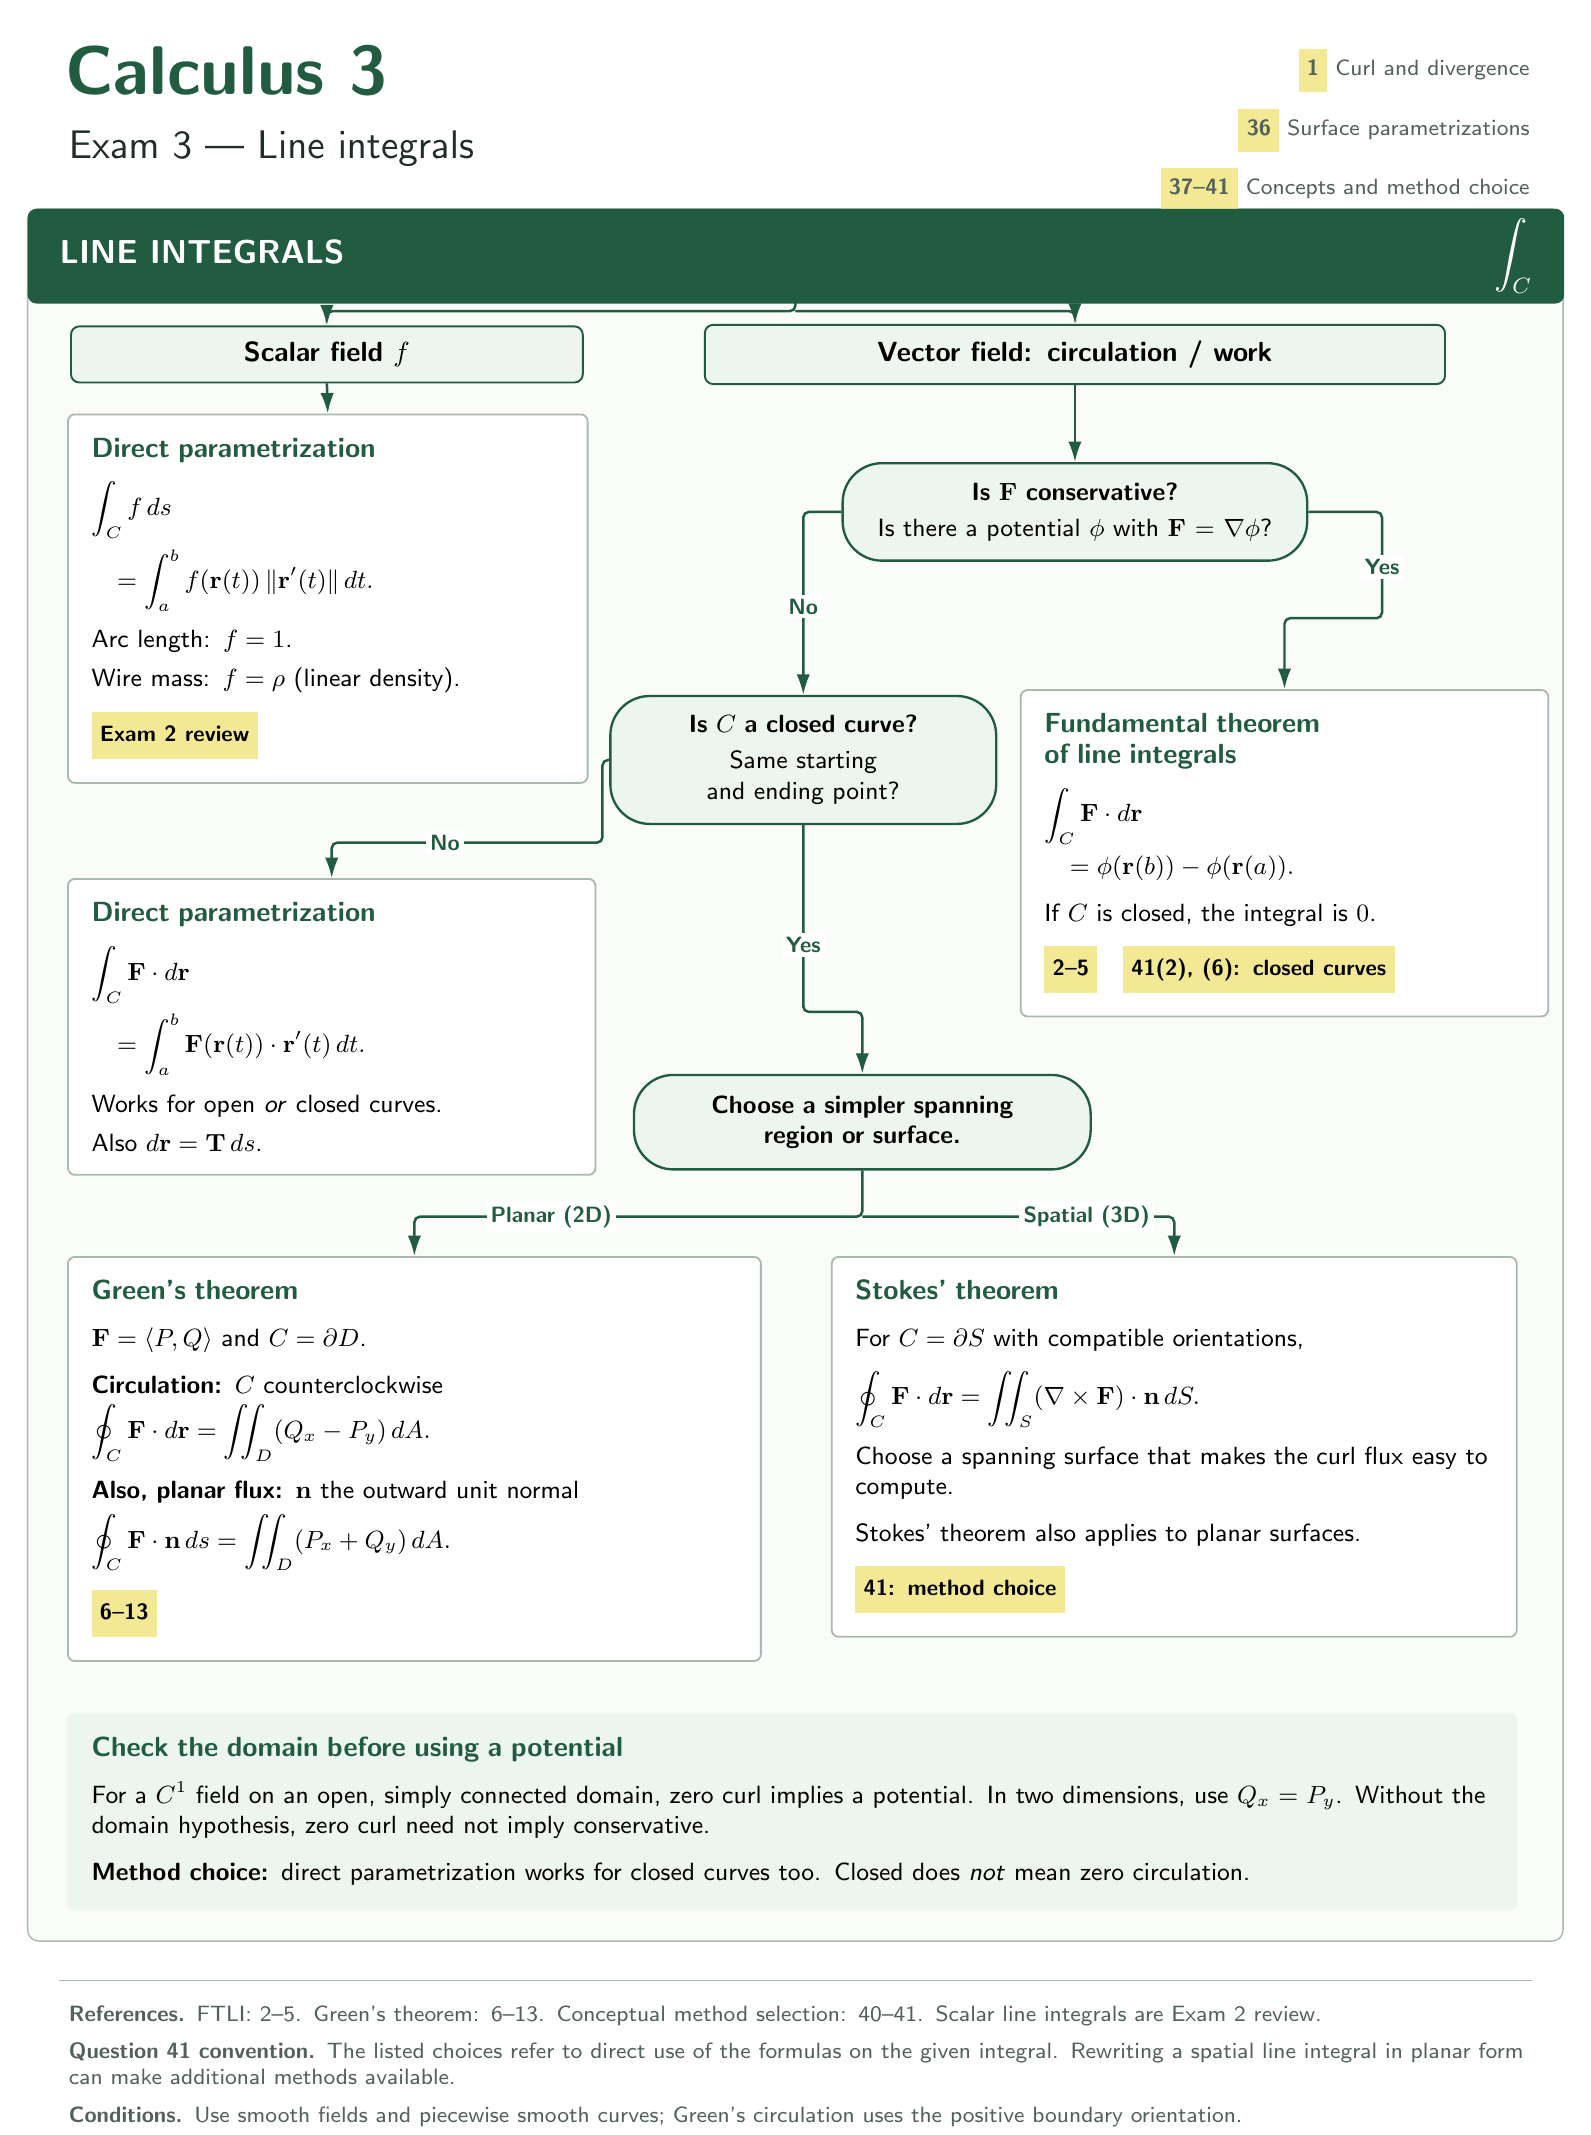
\begin{tikzpicture}[x=1cm,y=-1cm,font=\sffamily\small]
  \path[use as bounding box] (0,0) rectangle (19.5,26.4);
  \node[anchor=north west,font=\sffamily\bfseries\fontsize{27}{30}\selectfont,text=Green]
    at (.35,.12) {Calculus 3};
  \node[anchor=north west,font=\sffamily\fontsize{15}{18}\selectfont,text=Ink]
    at (.4,1.18) {Exam 3 | Line integrals};
  \node[anchor=north east,align=right,font=\sffamily\footnotesize,text=Muted]
    at (19.2,.15) {\qtag{1}\ Curl and divergence\\[5pt]
      \qtag{36}\ Surface parametrizations\\[5pt]
      \qtag{37--41}\ Concepts and method choice};
  \begin{scope}[on background layer]
    \filldraw[fill=Panel,draw=Rule,line width=.5pt,rounded corners=4pt]
      (0,2.3) rectangle (19.5,24.3);
  \end{scope}
  \node[panelhead,text width=18.7cm] (Lhead) at (0,2.3)
    {LINE INTEGRALS \hfill $\displaystyle\int_C$};

  \node[type,text width=6.1cm] (Lscalar) at (3.8,4.15) {Scalar field $f$};
  \node[type,text width=9cm] (Lvector) at (13.3,4.15) {Vector field: circulation / work};
  \draw[flow] (9.75,3.2) -- (9.75,3.6) -| (Lscalar.north);
  \draw[flow] (9.75,3.6) -| (Lvector.north);

  \node[card,text width=6cm,minimum height=3.6cm] (Lscalarformula) at (.5,4.9) {
    \cardtitle{Direct parametrization}
    $\displaystyle\int_C f\,ds$
    \par\smallskip
    $\displaystyle\quad=\int_a^b f(\rr(t))\,\|\rr'(t)\|\,dt.$
    \par\medskip
    Arc length: $f=1$.\\[3pt]
    Wire mass: $f=\rho$ (linear density).
    \par\medskip
    \qtag{Exam 2 review}
  };
  \draw[flow] (Lscalar.south) -- (Lscalarformula.north);

  \node[decision,text width=5.3cm] (conservative) at (13.3,6.15) {
    \textbf{Is $\F$ conservative?}\\[2pt]
    Is there a potential $\phi$ with $\F=\nabla\phi$?
  };
  \draw[flow] (Lvector.south) -- (conservative.north);

  \node[decision,text width=4.3cm] (closedcurve) at (9.85,9.3) {
    \textbf{Is $C$ a closed curve?}\\[2pt]
    Same starting and ending point?
  };
  \draw[flow] (conservative.west) -- (9.85,6.15) -- (closedcurve.north);
  \node[branch] at (9.85,7.35) {No};

  \node[card,text width=6.1cm,minimum height=3.6cm] (ftoli) at (12.6,8.4) {
    \cardtitle{Fundamental theorem\\of line integrals}
    $\displaystyle\int_C\F\cdot d\rr$
    \par\smallskip
    $\displaystyle\quad=\phi(\rr(b))-\phi(\rr(a)).$
    \par\medskip
    If $C$ is closed, the integral is $0$.
    \par\medskip
    \qtag{2--5}\quad\qtag{41(2), (6): closed curves}
  };
  \draw[flow] (conservative.east) -- (17.2,6.15) -- (17.2,7.5)
    -| (ftoli.north);
  \node[branch] at (17.2,6.85) {Yes};

  \node[card,text width=6.1cm,minimum height=3.1cm] (Ldirect) at (.5,10.8) {
    \cardtitle{Direct parametrization}
    $\displaystyle\int_C\F\cdot d\rr$
    \par\smallskip
    $\displaystyle\quad=\int_a^b\F(\rr(t))\cdot\rr'(t)\,dt.$
    \par\medskip
    Works for open \emph{or} closed curves.\\[3pt]
    Also $d\rr=\TT\,ds$.
  };
  \draw[flow] (closedcurve.west) -- (7.3,9.3) -- (7.3,10.35) -| (Ldirect.north);
  \node[branch] at (5.3,10.35) {No};

  \node[decision,text width=5.2cm] (spanning) at (10.6,13.9) {
    \textbf{Choose a simpler spanning\\region or surface.}
  };
  \draw[flow] (closedcurve.south) -- (9.85,12.5) -| (spanning.north);
  \node[branch] at (9.85,11.65) {Yes};

  \node[card,text width=8.2cm,minimum height=4.75cm] (green) at (.5,15.6) {
    \cardtitle{Green's theorem}
    $\F=\langle P,Q\rangle$ and $C=\partial D$.
    \par\medskip
    \textbf{Circulation:} $C$ counterclockwise
    \par\smallskip
    $\displaystyle\oint_C\F\cdot d\rr
       =\iint_D(Q_x-P_y)\,dA.$
    \par\medskip
    \textbf{Also, planar flux:} $\nn$ the outward unit normal
    \par\smallskip
    $\displaystyle\oint_C\F\cdot\nn\,ds
       =\iint_D(P_x+Q_y)\,dA.$
    \par\medskip
    \qtag{6--13}
  };
  \node[card,text width=8.1cm,minimum height=3.8cm] (Lstokes) at (10.2,15.6) {
    \cardtitle{Stokes' theorem}
    For $C=\partial S$ with compatible orientations,
    \par\medskip
    $\displaystyle\oint_C\F\cdot d\rr
      =\iint_S(\curl\F)\cdot\nn\,dS.$
    \par\medskip
    Choose a spanning surface that makes the curl flux easy to compute.
    \par\medskip
    Stokes' theorem also applies to planar surfaces.\par\medskip
    \qtag{41: method choice}
  };
  \draw[flow] (spanning.south) -- (10.6,15.1) -| (green.north);
  \draw[flow] (10.6,15.1) -| (Lstokes.north);
  \node[branch] at (6.65,15.1) {Planar (2D)};
  \node[branch] at (13.45,15.1) {Spatial (3D)};

  \node[note,text width=17.8cm,minimum height=2.35cm] (Lnote) at (.5,21.4) {
    \cardtitle{Check the domain before using a potential}
    For a $C^1$ field on an open, simply connected domain, zero curl implies a potential.
    In two dimensions, use $Q_x=P_y$. Without the domain hypothesis, zero curl need not imply conservative.
    \par\medskip
    \textbf{Method choice:} direct parametrization works for closed curves too. Closed does \emph{not} mean zero circulation.
  };

  \draw[Rule,line width=.6pt] (.4,24.8) -- (19.1,24.8);
  \node[anchor=north west,text width=18.7cm,align=left,font=\sffamily\footnotesize,text=Muted]
    at (.4,25.0) {
      \textbf{References.} FTLI: 2--5. Green's theorem: 6--13.
      Conceptual method selection: 40--41. Scalar line integrals are Exam 2 review.
      \\[4pt]
      \textbf{Question 41 convention.} The listed choices refer to direct use of the formulas on the given integral.
      Rewriting a spatial line integral in planar form can make additional methods available.
      \\[4pt]
      \textbf{Conditions.} Use smooth fields and piecewise smooth curves; Green's circulation uses the positive boundary orientation.
    };
\end{tikzpicture}%
}
\end{center}

\clearpage
\begin{center}
\resizebox{!}{0.98\textheight}{%
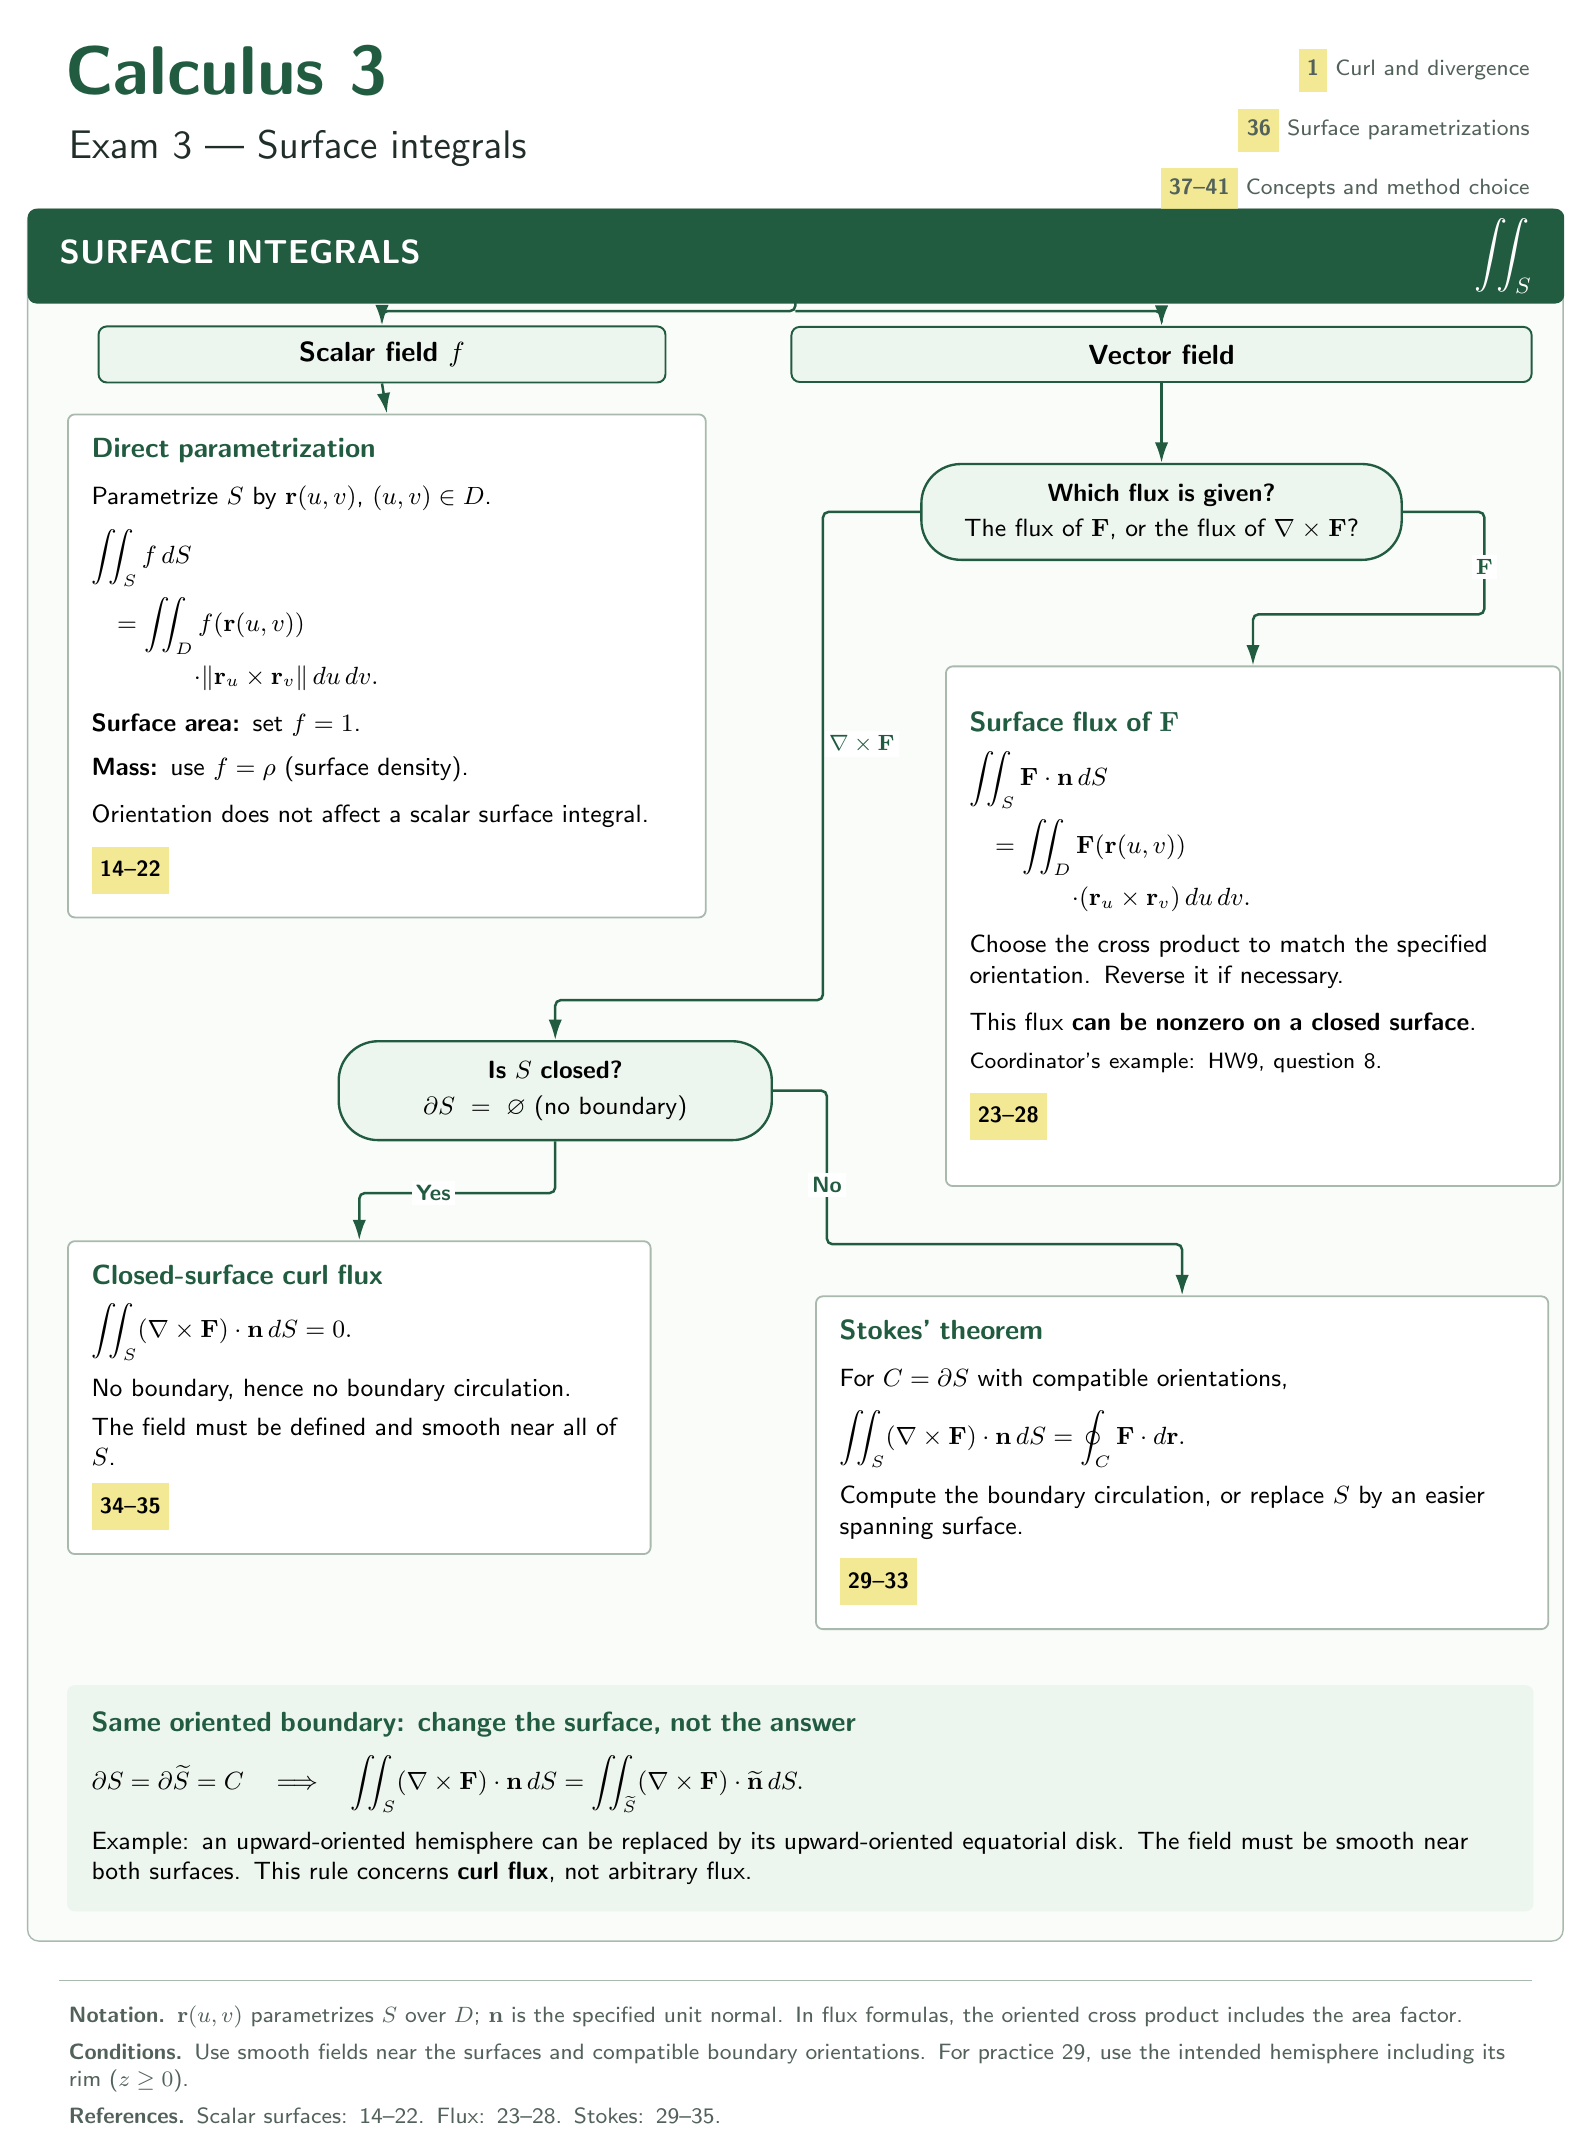
\begin{tikzpicture}[x=1cm,y=-1cm,font=\sffamily\small]
  \path[use as bounding box] (0,0) rectangle (19.5,26.4);
  \node[anchor=north west,font=\sffamily\bfseries\fontsize{27}{30}\selectfont,text=Green]
    at (.35,.12) {Calculus 3};
  \node[anchor=north west,font=\sffamily\fontsize{15}{18}\selectfont,text=Ink]
    at (.4,1.18) {Exam 3 | Surface integrals};
  \node[anchor=north east,align=right,font=\sffamily\footnotesize,text=Muted]
    at (19.2,.15) {\qtag{1}\ Curl and divergence\\[5pt]
      \qtag{36}\ Surface parametrizations\\[5pt]
      \qtag{37--41}\ Concepts and method choice};
  \begin{scope}[shift={(-20,0)}]
  \begin{scope}[on background layer]
    \filldraw[fill=Panel,draw=Rule,line width=.5pt,rounded corners=4pt]
      (20,2.3) rectangle (39.5,24.3);
  \end{scope}
  \node[panelhead,text width=18.7cm] (Rhead) at (20,2.3)
    {SURFACE INTEGRALS \hfill $\displaystyle\iint_S$};

  \node[type,text width=6.8cm] (Rscalar) at (24.5,4.15) {Scalar field $f$};
  \node[type,text width=9cm] (Rvector) at (34.4,4.15) {Vector field};
  \draw[flow] (29.75,3.2) -- (29.75,3.6) -| (Rscalar.north);
  \draw[flow] (29.75,3.6) -| (Rvector.north);

  \node[card,text width=7.5cm,minimum height=5.65cm] (Rscalarformula) at (20.5,4.9) {
    \cardtitle{Direct parametrization}
    Parametrize $S$ by $\rr(u,v)$, $(u,v)\in D$.
    \par\medskip
    $\displaystyle\iint_S f\,dS$
    \par\smallskip
    $\displaystyle\quad=\iint_D f(\rr(u,v))$
    \par\smallskip
    $\displaystyle\qquad\qquad\cdot\|\rr_u\times\rr_v\|\,du\,dv.$
    \par\medskip
    \textbf{Surface area:} set $f=1$.\\[5pt]
    \textbf{Mass:} use $f=\rho$ (surface density).
    \par\medskip
    Orientation does not affect a scalar surface integral.
    \par\medskip
    \qtag{14--22}
  };
  \draw[flow] (Rscalar.south) -- (Rscalarformula.north);

  \node[decision,text width=5.5cm] (whichflux) at (34.4,6.15) {
    \textbf{Which flux is given?}\\[2pt]
    The flux of $\F$, or the flux of $\nabla\times\F$?
  };
  \draw[flow] (Rvector.south) -- (whichflux.north);

  \node[card,text width=7.2cm,minimum height=6.6cm] (Rflux) at (31.65,8.1) {
    \cardtitle{Surface flux of $\F$}
    $\displaystyle\iint_S\F\cdot\nn\,dS$
    \par\smallskip
    $\displaystyle\quad=\iint_D\F(\rr(u,v))$
    \par\smallskip
    $\displaystyle\qquad\qquad\cdot(\rr_u\times\rr_v)\,du\,dv.$
    \par\medskip
    Choose the cross product to match the specified orientation. Reverse it if necessary.
    \par\medskip
    This flux \textbf{can be nonzero on a closed surface}.
    \par\smallskip
    {\footnotesize Coordinator's example: HW9, question 8.}
    \par\medskip
    \qtag{23--28}
  };
  \draw[flow] (whichflux.east) -- (38.5,6.15) -- (38.5,7.45) -| (Rflux.north);
  \node[branch] at (38.5,6.85) {$\F$};

  \node[decision,text width=4.9cm] (closedsurface) at (26.7,13.5) {
    \textbf{Is $S$ closed?}\\[2pt]
    $\partial S=\varnothing$ (no boundary)
  };
  \draw[flow] (whichflux.west) -- (30.1,6.15) -- (30.1,12.35)
    -| (closedsurface.north);
  \node[branch,anchor=west] at (30.12,9.1) {$\nabla\times\F$};

  \node[card,text width=6.8cm,minimum height=2.65cm] (zero) at (20.5,15.4) {
    \cardtitle{Closed-surface curl flux}
    $\displaystyle\iint_S(\curl\F)\cdot\nn\,dS=0.$
    \par\medskip
    No boundary, hence no boundary circulation.
    \par\smallskip
    The field must be defined and smooth near all of $S$.\par\medskip
    \qtag{34--35}
  };
  \draw[flow] (closedsurface.south) -- (26.7,14.8) -| (zero.north);
  \node[branch] at (25.15,14.8) {Yes};

  \node[card,text width=8.7cm,minimum height=3.7cm] (Rstokes) at (30.0,16.1) {
    \cardtitle{Stokes' theorem}
    For $C=\partial S$ with compatible orientations,
    \par\medskip
    $\displaystyle\iint_S(\curl\F)\cdot\nn\,dS
       =\oint_C\F\cdot d\rr.$
    \par\medskip
    Compute the boundary circulation, or replace $S$ by an easier spanning surface.
    \par\medskip
    \qtag{29--33}
  };
  \draw[flow] (closedsurface.east) -- (30.15,13.5) -- (30.15,15.45)
    -| (Rstokes.north);
  \node[branch] at (30.15,14.7) {No};

  \node[note,text width=18cm,minimum height=2.85cm] (Rnote) at (20.5,21.05) {
    \cardtitle{Same oriented boundary: change the surface, not the answer}
    $\displaystyle\partial S=\partial\widetilde S=C
      \quad\Longrightarrow\quad
      \iint_S(\curl\F)\cdot\nn\,dS
      =\iint_{\widetilde S}(\curl\F)\cdot\widetilde\nn\,dS.$
    \par\medskip
    Example: an upward-oriented hemisphere can be replaced by its upward-oriented equatorial disk.
    The field must be smooth near both surfaces. This rule concerns \textbf{curl flux}, not arbitrary flux.
  };

  \end{scope}
  \draw[Rule,line width=.6pt] (.4,24.8) -- (19.1,24.8);
  \node[anchor=north west,text width=18.7cm,align=left,font=\sffamily\footnotesize,text=Muted]
    at (.4,25.0) {
      \textbf{Notation.} $\rr(u,v)$ parametrizes $S$ over $D$; $\nn$ is the specified unit normal.
      In flux formulas, the oriented cross product includes the area factor.
      \\[4pt]
      \textbf{Conditions.} Use smooth fields near the surfaces and compatible boundary orientations.
      For practice 29, use the intended hemisphere including its rim ($z\ge0$).
      \\[4pt]
      \textbf{References.} Scalar surfaces: 14--22. Flux: 23--28. Stokes: 29--35.
    };
\end{tikzpicture}%
}
\end{center}

\clearpage

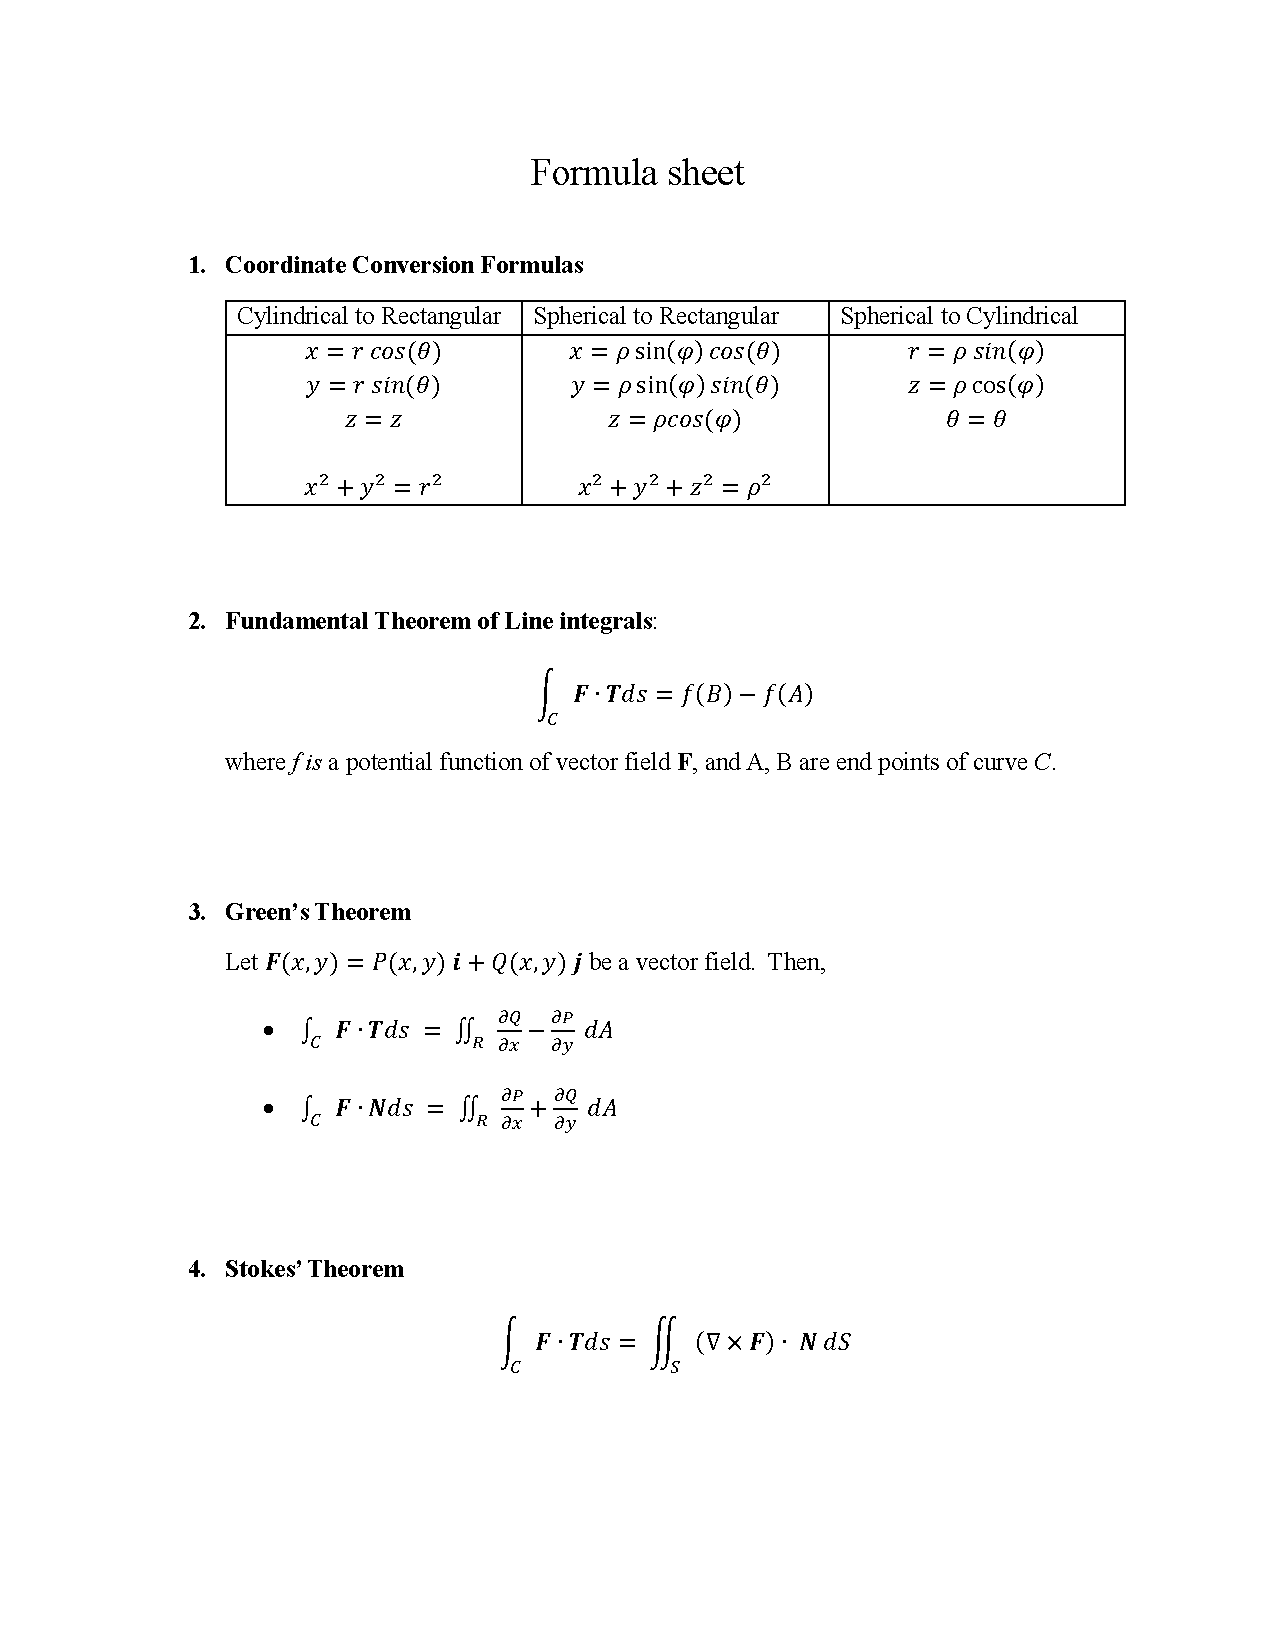
\includepdf[pages=-,fitpaper=false]{e3.pdf}
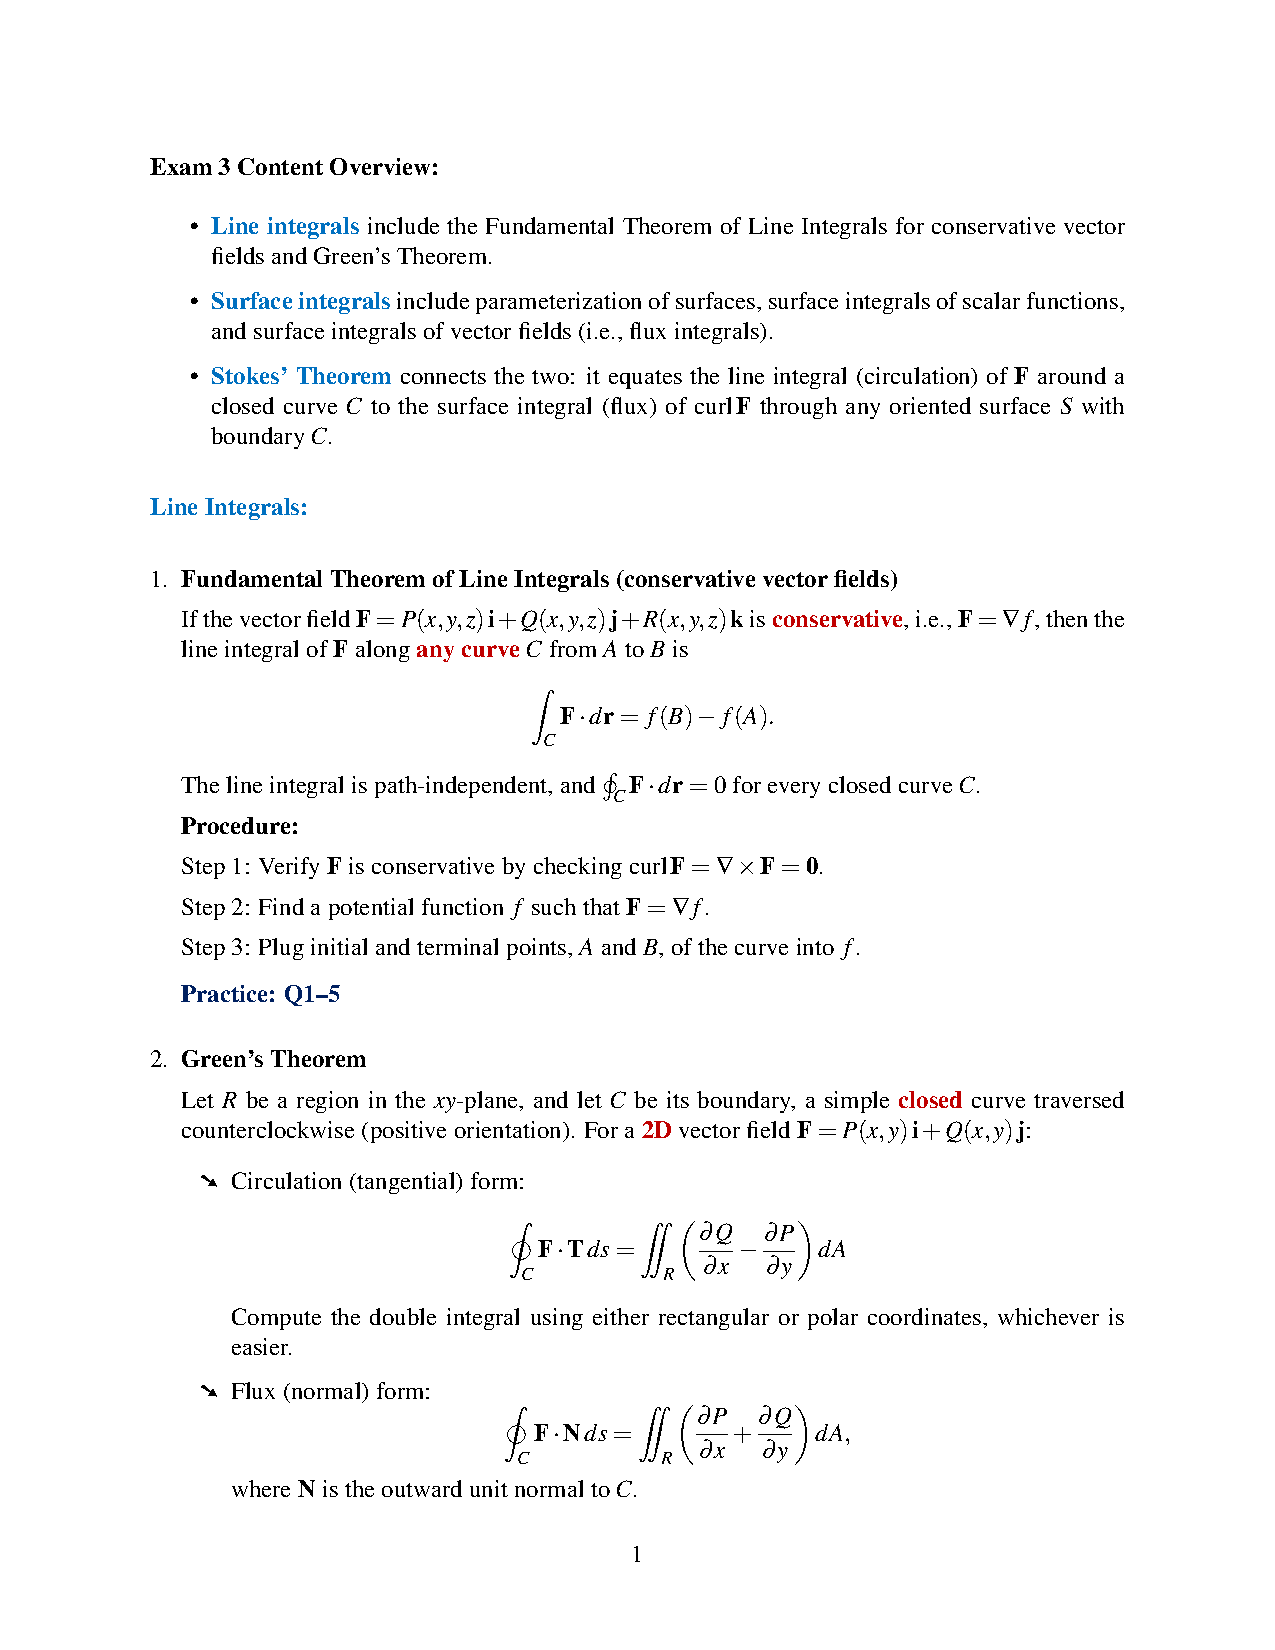
\includepdf[pages=-,fitpaper=false]{e31.pdf}
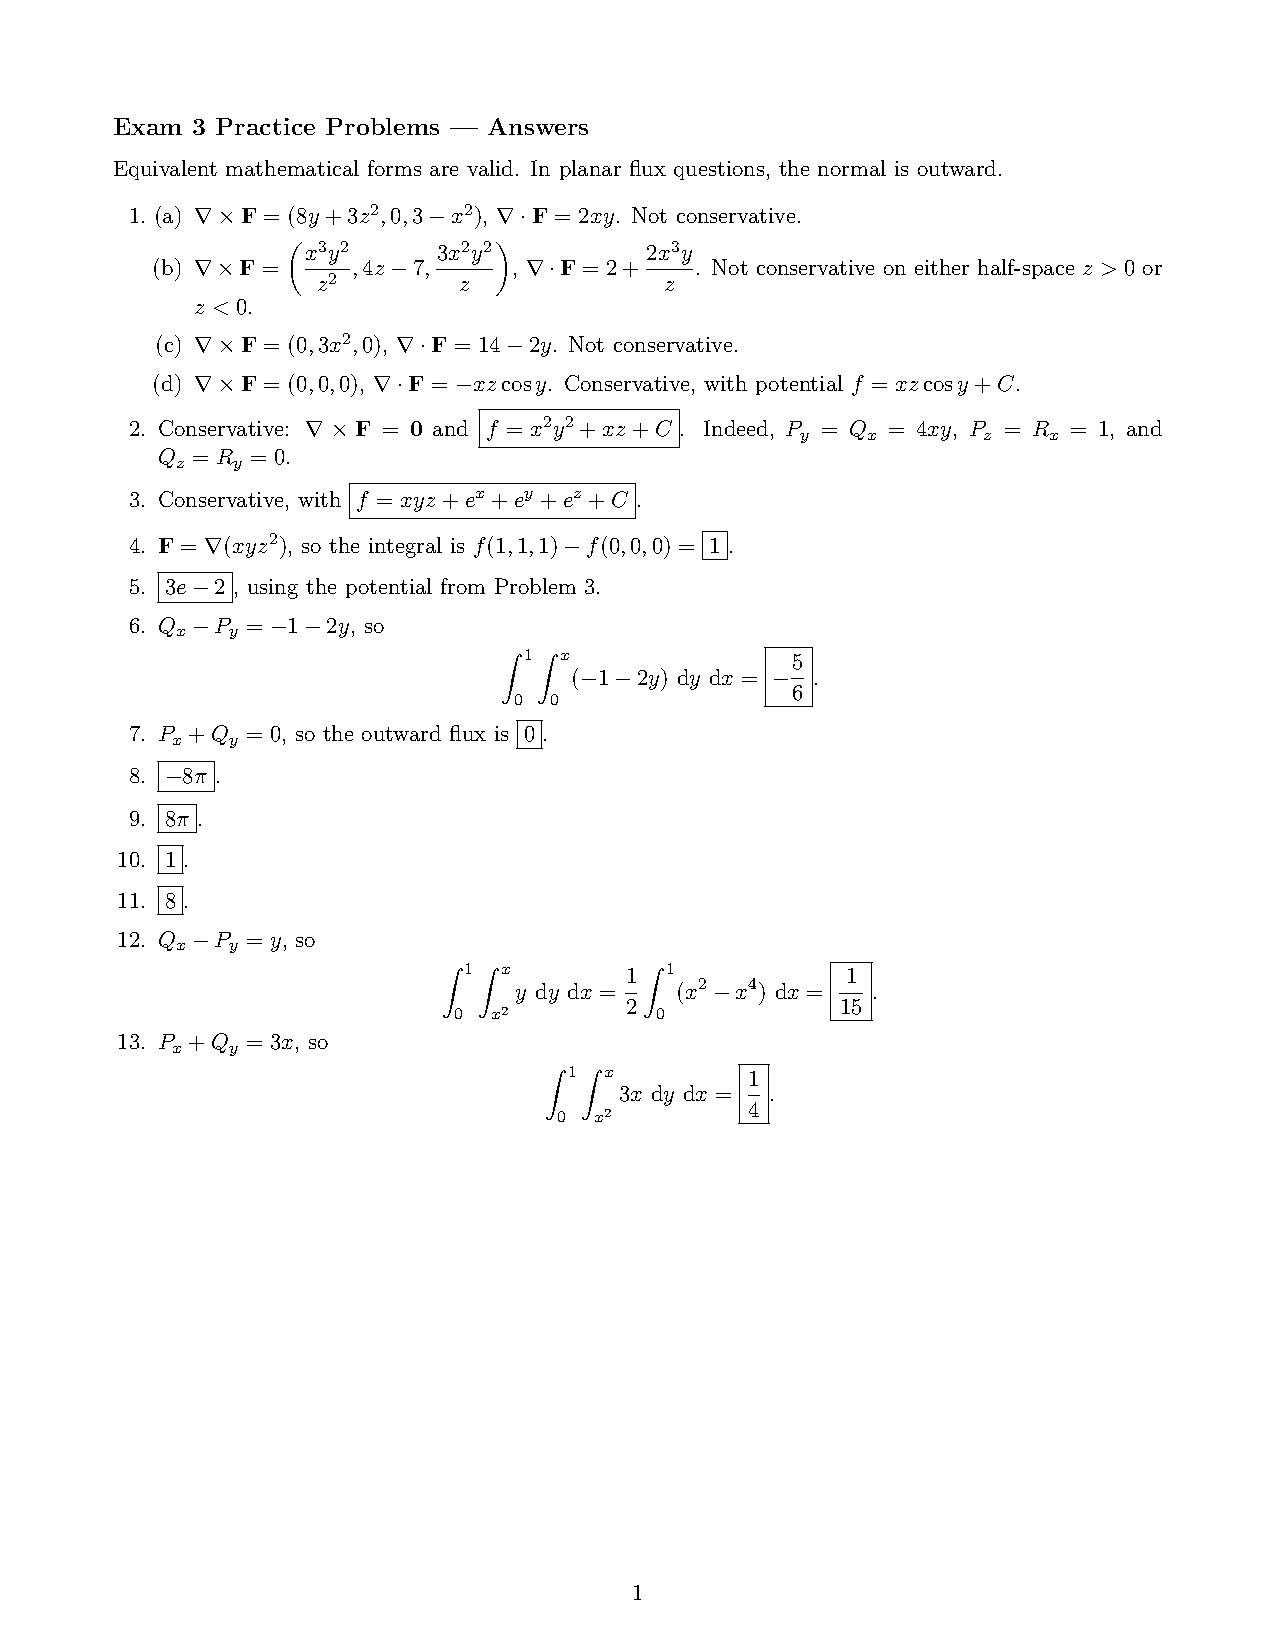
\includepdf[pages=-,fitpaper=false]{e32-corrected.pdf}
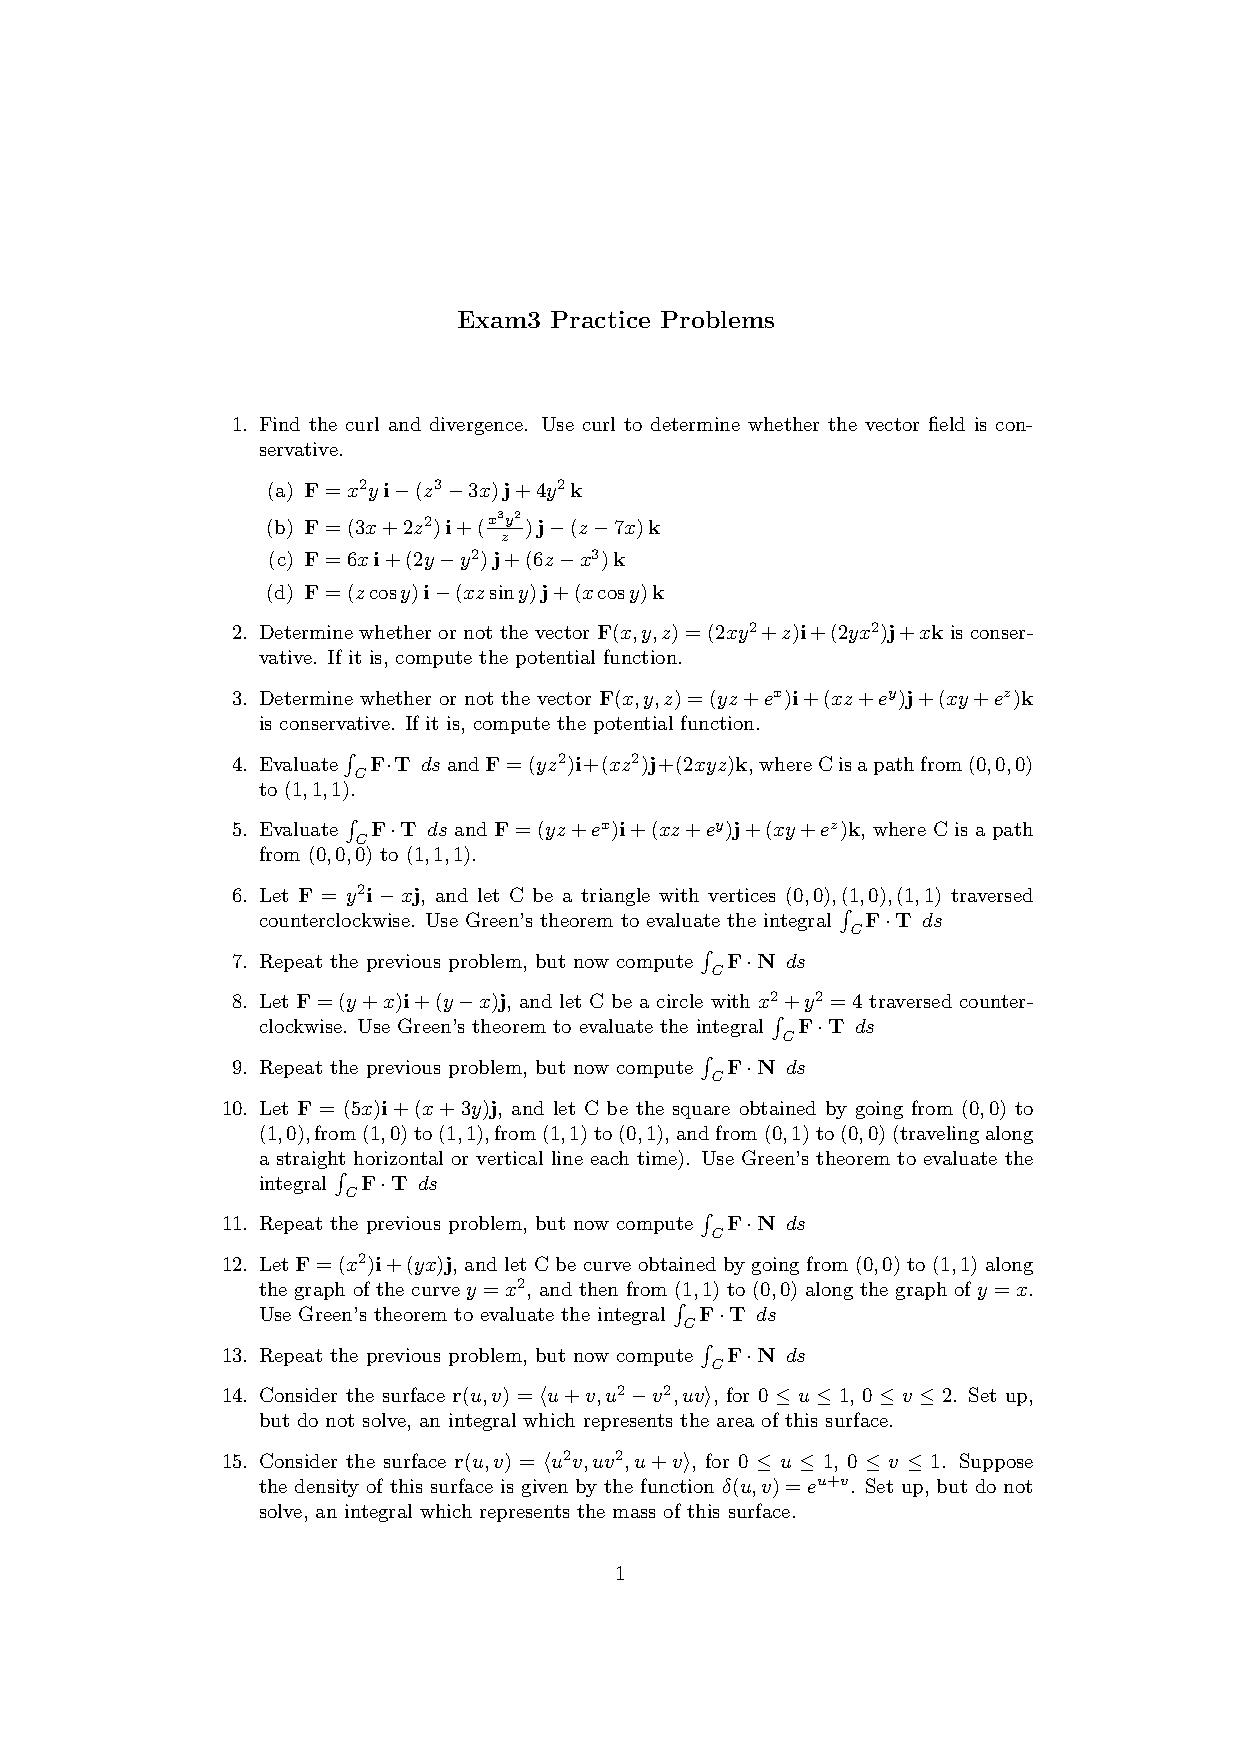
\includepdf[pages=-,fitpaper=false]{e33.pdf}
\end{document}
